% !TeX program = xelatex
%% 부득이하게 pdflatex을 사용해야 할 경우 위의 magic comment를 제거하십시오.

%%%%%%%%%%%%%%%%%%%%%%%%%%%%%%%%%%%%%%%%%%%%%%%%%%%%%%%%%%%%%%%%%%%%%%%%%%%%%%%%%
%%%  LaTeX document class of the thesis of the Gyeonggi Science High School   %%%
%%%  Last edition 2015.11.13 by Chinook Mok                                   %%%
%%%  Continously being modified by gshslatexintro after 2016.02.02.           %%%
%%%  Check the latest version at : latex.gs.hs.kr                             %%%
%%%  Also refer to https://www.facebook.com/gshstexsociety                    %%%
%%%%%%%%%%%%%%%%%%%%%%%%%%%%%%%%%%%%%%%%%%%%%%%%%%%%%%%%%%%%%%%%%%%%%%%%%%%%%%%%%

\documentclass{gshs_thesis}

\graphicspath{{images/}}
% 이곳에 필요한 별도의 패키지들을 적어넣으시오.
%\usepackage{...}
\usepackage{verbatim} % for commment, verbatim environment
\usepackage{spverbatim} % automatic linebreak verbatim environment
%\usepacakge{indentfirst}
\usepackage{listings}
\lstset{
	basicstyle=\small\ttfamily,
	columns=flexible,
	breaklines=true
}
\usepackage{hologo}

\citation
\bibdata

% -----------------------------------------------------------------------
%                   이 부분은 수정하지 마시오.
% -----------------------------------------------------------------------
\titleheader{졸업논문청구논문}
\school{과학영재학교 경기과학고등학교}
\approval{위 논문은 과학영재학교 경기과학고등학교 졸업논문으로\\
졸업논문심사위원회에서 심사 통과하였음.}
\chairperson{심사위원장}
\examiner{심사위원}
\apprvsign{(인)}
\korabstract{초 록}
\koracknowledgement{감사의 글}
\korresearches{연 구 활 동}

%: ----------------------------------------------------------------------
%:                  논문 제목과 저자 이름을 입력하시오
% ----------------------------------------------------------------------
\title{SeaWiFS 해색 자료를 이용한 동해에서의 chlorophyll-a 농도 분석 : LAC 자료와 GAC 자료의 비교} %한글 제목
\engtitle{Analysis of the chlorophyll-a concentration in the Korean East Sea using SeaWiFS ocean color data : comparison between the LAC data and the GAC data} %영문 제목
\korname{김 병 현} %저자 이름을 한글로 입력하시오 (글자 사이 띄어쓰기)
\engname{Kim, Byung Hyun} %저자 이름을 영어로 입력하시오 (family name, personal name)
\chnname{金 柄 賢} %저자 이름을 한자로 입력하시오 (글자 사이 띄어쓰기)
\studid{15021} %학번을 입력하시오

%------------------------------------------------------------------------
%                  심사위원과 논문 승인 날짜를 입력하시오
%------------------------------------------------------------------------
\advisor{Park, Kie Hyun}  %지도교사 영문 이름 (family name, personal name)
\judgeone{박 경 애} %심사위원장
\judgetwo{김 학 성}   %심사위원1
\judgethree{박 기 현} %심사위원2(지도교사)
\degreeyear{2017}   %졸업 년도
\degreedate{2017}{11}{13} %논문 승인 날짜 양식

%------------------------------------------------------------------------
%                  논문제출 전 체크리스트를 확인하시오
%------------------------------------------------------------------------
\checklisttitle{[논문제출 전 체크리스트]} %수정하지 마시오
\checklistI{1. 이 논문은 내가 직접 연구하고 작성한 것이다.} %수정하지 마시오
% 이 항목이 사실이라면 다음 줄 앞에 "%"기호 삽입, 다다음 줄 앞의 "%"기호 제거하시오
\checklistmarkI{$\square$}
%\checklistmarkI{$\text{\rlap{$\checkmark$}}\square$}
\checklistII{2. 인용한 모든 자료(책, 논문, 인터넷자료 등)의 인용표시를 바르게 하였다.} %수정하지 마시오
% 이 항목이 사실이라면 다음 줄 앞에 "%"기호 삽입, 다다음 줄 앞의 "%"기호 제거하시오
\checklistmarkII{$\square$}
%\checklistmarkII{$\text{\rlap{$\checkmark$}}\square$}
\checklistIII{3. 인용한 자료의 표현이나 내용을 왜곡하지 않았다.} %수정하지마시오
% 이 항목이 사실이라면 다음 줄 앞에 "%"기호 삽입, 다다음 줄 앞의 "%"기호 제거하시오
\checklistmarkIII{$\square$}
%\checklistmarkIII{$\text{\rlap{$\checkmark$}}\square$}
\checklistIV{4. 정확한 출처제시 없이 다른 사람의 글이나 아이디어를 가져오지 않았다.} %수정하지 마시오
% 이 항목이 사실이라면 다음 줄 앞에 "%"기호 삽입, 다다음 줄 앞의 "%"기호 제거하시오
\checklistmarkIV{$\square$}
%\checklistmarkIV{$\text{\rlap{$\checkmark$}}\square$}
\checklistV{5. 논문 작성 중 도표나 데이터를 조작(위조 혹은 변조)하지 않았다.} %수정하지 마시오
% 이 항목이 사실이라면 다음 줄 앞에 "%"기호 삽입, 다다음 줄 앞의 "%"기호 제거하시오
\checklistmarkV{$\square$}
%\checklistmarkV{$\text{\rlap{$\checkmark$}}\square$}
\checklistVI{6. 다른 친구와 같은 내용의 논문을 제출하지 않았다.} %수정하지 마시오
% 이 항목이 사실이라면 다음 줄 앞에 "%"기호 삽입, 다다음 줄 앞의 "%"기호 제거하시오
\checklistmarkVI{$\square$}
%\checklistmarkVI{$\text{\rlap{$\checkmark$}}\square$} % usepackage 등의 명령어는 여기에.

\usepackage{tocloft}
\setlength{\cftbeforesecskip}{0pt}
\setlength{\cftbeforesubsecskip}{0pt}
\setlength{\cftbeforesubsubsecskip}{0pt}

\begin{document}
%	\renewcommand\baselinestretch{1.2} % line spacing in the paragraph
	\baselineskip=2.2em         % line spacing in the paragraph
	
	\maketitle  % command to print the title page with above variables

\setcounter{page}{1}
%---------------------------------------------------------------------
%                  영문 초록을 입력하시오
%---------------------------------------------------------------------
\begin{abstracts}     %this creates the heading for the abstract page
	\addcontentsline{toc}{section}{Abstract}  %%% TOC에 표시
	\noindent{
		다시 번역
		The seasonal variability chlorophyll-a concentration in the Korean East Sea had been obtained by processing SeaWiFS Local Area Coverage(LAC) and Global Area Coverage(GAC) oceancolor data from January 2003 to December 2006. Both data showed similarities in the tendency showing peaks on spring(April) and fall(November). However, the value of chlorophyll-a concentration was different, the maximum/minimum value of LAC and GAC data each being 1.61 mg/m3 / 0.28 mg/m3, and 1.72 mg/m3 / 0.32 mg/m3. Comparing the pixel histogram of LAC and GAC data showed GAC data had more speckle errors. The pixel analysis of chlorophyll-a concentration data on April, 2003 also showed it is more accurate to use LAC data because of its high resolution.
	}
\end{abstracts}

%---------------------------------------------------------------------
%                  국문 초록을 입력하시오
%---------------------------------------------------------------------
\begin{abstractskor}        %this creates the heading for the abstract page
	\addcontentsline{toc}{section}{초록}  %%% TOC에 표시
	\noindent{
SeaWiFS LAC (Local Area Coverage) 및 GAC (Global Area Coverage) 자료를 이용하여 2003년 1월부터 2006년 12월까지 동해의 chlorophyll-a 월평균 농도를 산출하였다. 두 자료 모두 봄철(4월)과 가을철(11월)에 월평균 농도가 높게 산출되어 전체적인 경향은 비슷하게 나타났다. 그러나 LAC와 GAC 자료로 산출한 chlorophyll-a 월평균 농도의 최대값/최소값은 각각 1.61 $\rm mg/m^3$ / 0.28 $\rm mg/m^3$ 과 1.72 $\rm mg/m^3$ / 0.32 $\rm mg/m^3$으로 차이가 나타났다. 차이를 구체적으로 분석하기 위하여 LAC와 GAC 데이터의 픽셀 히스토그램을 비교한 결과 GAC 데이터에서 스펙클 오류가 더 크게 나타남을 확인하였다. Chlorophyll-a 월평균 농도가 높았던 2003년 4월 이미지 픽셀을 분석해 본 결과 해상도가 높은 LAC 자료를 이용하는 것이 GAC 자료를 이용하는 것 보다 더 정확함을 확인하였다. 
	}
\end{abstractskor}

%----------------------------------------------
%   Table of Contents (자동 작성됨)
%----------------------------------------------
\cleardoublepage
\addcontentsline{toc}{section}{Contents}
\setcounter{secnumdepth}{3} % organisational level that receives a numbers
\setcounter{tocdepth}{3}    % print table of contents for level 3
\baselineskip=2.2em
\tableofcontents


%----------------------------------------------
%     List of Figures/Tables (자동 작성됨)
%----------------------------------------------
\cleardoublepage
\clearpage
\listoftables
% 표 목록과 캡션을 출력한다. 만약 논문에 표가 없다면 이 위 줄의 맨 앞에 
% `%' 기호를 넣어서 주석 처리한다.

\cleardoublepage
\clearpage
\listoffigures
% 그림 목록과 캡션을 출력한다. 만약 논문에 그림이 없다면 이 위 줄의 맨 앞에 
% `%' 기호를 넣어서 주석 처리한다.

\cleardoublepage
\clearpage
\listofequations
% 그림 목록과 캡션을 출력한다. 만약 논문에 그림이 없다면 이 위 줄의 맨 앞에 
% `%' 기호를 넣어서 주석 처리한다.


\cleardoublepage
\clearpage
\renewcommand{\thepage}{\arabic{page}}
\setcounter{page}{1} % Abstract

	%%%%%%%%%%%%%%%%%%%%%%%%%%%%%%%%%%%%%%%%%%%%%%%%%%%%%%%%%%%
	%%%% Main Document %%%%%%%%%%%%%%%%%%%%%%%%%%%%%%%%%%%%%%%%
	%%%%%%%%%%%%%%%%%%%%%%%%%%%%%%%%%%%%%%%%%%%%%%%%%%%%%%%%%%%

	\section{Introduction}

Algae is an important factor in the marine ecosystem. It adds oxygen to water by photosynthesis, and it also determines the water transparency. However, when nutrients are oversupplied, eutrophication occurs causing overgrowth of algae in water. Such phenomenon is called as algal bloom. It blocks sunlight and also consumes lot of oxygen when it dies and decomposes, causing a negative effect on the marine environment. In addition, measuring the amount of algae in the water is crucial.

Ocean color remote sensing allows us to indirectly measure various matters in the ocean. The Coastal Zone Color Scanner (CZCS) that is the first ocean colour sensor, operated from 1978 to 1986 and the Sea-viewing Wide Field-of-view Sensor (SeaWiFS) has observed global ocean colour distributions for about a decade, from 1998 to 2010, and has provided the scientific community with abundant information for a variety of oceanic application research \cite{kyung2013characteristics, hooker1992An}.

It collects several bands of reflected light from the ocean, which can be calculated to amount of matters using developed algorithms. The data we obtain from such methods is called ocean color data. Ocean color data is important in understanding the temporal and spatial distribution of algae \cite{kimhc2016surface}.

Chlorophyll-a concentration can be calculated using ocean color remote sensing. Since chlorophyll-a is a pigment that is required for photosynthesis, it is also found in algae. Additionally, chlorophyll-a concentration is used as a determinant for the amount of algae in ocean \cite{o2000ocean}. 

There have been several studies about chlorophyll-a concentration in the Korean East Sea, using ocean color remote sensing. Spring bloom and fall bloom were observed, showing a seasonal pattern. The chlorophyll-a concentration was also found to be related with wind, sea surface temperature, and many other variables of the ocean \cite{yamada2004seasonal}. SeaWiFS(Sea-Viewing Wide Field-of-View Sensor) satellite is often used for studying the chlorophyll-a concentration in the Korean East Sea. It was found to have small areas with abnormally high concentration of chlorophyll-a compared to the areas nearby, which is called speckles. There had been studies to correct this error \cite{chae2009characteristics}. 

SeaWiFS creates two types of level 1 data with different spatial resolutions, Local-Area Coverage(LAC) data and Global-Area Coverage(GAC) data. Level-1 data is a data that had gone through radiometric and geometric calibration. LAC is created with full-resolution(1.1km) for local area while GAC is created with low resolution(4.5km) for a global area. They both use the OC4 algorithm and the color index algorithm to be converted to level-2 chlorophyll-a concentration data. Level-2 data is a data of geophysical variables processed from level-1 data. 

(LAC와 GAC 차이를 좀 더 자세히 적고 인용표시)

Although many scientists used SeaWiFS LAC data and GAC data for research, they did not found which is more suitable. There is also no proof that applying same algorithms will give both accurate results. 

The goal of this research are the followings. First, observing the chlorophyll-a concentration variability in the Korean East Sea from 2003 to 2006 using SeaWiFS ocean color data. Second, comparing the chlorophyll-a concentration data of LAC and GAC to find the effect of spatial resolution.

 % Introduction
	\section{Methodology}

\subsection{Acquiring SeaWiFS data}

 This research used SeaWiFS ocean color data to derive chlorophyll-a concentration since SeaWiFS is a satellite that was created to collect global ocean biological data. Moreover, SeaWiFS creates data with two different resolutions that can be compared. However, research on recent years is not possible since SeaWiFS had been activating from September 1997 to December 2010. Table \ref{table01} shows the mission charactoristics of SeaWiFS and Table \ref{table02} shows the Cahracteristics of the DeaWiFS ocean color sensor \cite{hooker1992An}.

 \begin{table}[h]\textwidth
 	\caption{The mission characteristics of SeaWiFS.}
 	\label{table01}
 	\centering
 	\begin{tabular}{c|c}
 		\hline \setlength{\arrayrulewidth}{0.8pt}. 
 	Orbit Type	& Sun Synchronous at 705 km \\ \hline
 	Equator Crossing &	Noon +20 min, descending \\ \hline
 	Orbital Period &	99 minutes  \\ \hline
 	Swath Width &	2,801 km LAC/HRPT (58.3 degrees)  \\ \hline
 	Swath Width &	1,502 km GAC (45 degrees)  \\ \hline
 	Spatial Resolution &	1.1 km LAC, 4.5 km GAC  \\ \hline
 	Real-Time Data Rate &	665 kbps  \\ \hline
 	Revisit Time &	1 day  \\ \hline
 	Digitization &	10 bits  \\ \hline
 	\end{tabular}
 \end{table}

 \begin{table}[h]\textwidth
	\caption{Cahracteristics of the DeaWiFS ocean color sensor.}
	\label{table02}
	\centering
	\begin{tabular}{c|c|c|c|c}
		\hline \setlength{\arrayrulewidth}{0.8pt}. 
		Band	& Wavelength FWHM[nm] & Saturation Radiance & Input Radiance & SNR\\ \hline
		1 & 402-422 & 13.63 & 9.10 & 499 \\ \hline
		2 & 433-453 & 13.25 & 8.41 & 674  \\ \hline
		3 & 480-500 & 10.50 & 6.56 & 667 \\ \hline
		4 & 500-520 & 9.08 & 5.64 & 640  \\ \hline
		5 & 545-565 & 7.44 & 4.57 & 596 \\ \hline
		6 & 660-680 & 4.20 & 2.46 & 442  \\ \hline
		7 & 745-785 & 3.00 & 1.61 & 455 \\ \hline
		8 & 845-885 & 2.13 & 1.09 & 467  \\ \hline

	\end{tabular}
\end{table}
 
 The SeaWiFS Level 2 data of chlorophyll-a was downloaded from NASA Ocean Color Web. Processing Level 1 data to Level 2 data was done by NASA, using NASA SeaDAS program. NASA SeaDAS uses two algorithms to create chlorophyll-a concentration data from the Level 1 data of remote sensing reflectance($\rm R_{rs}$); these algorithms are the OCx band ratio algorithm and the color index(CI) algorithm of Hu. 
 The OCx band ratio algorithm use the ratio of two bands in a fourth-order polynomial equation in a relation with chlorophyll-a It can be expressed as the following equation \ref{eq001}.
 
 \begin{equation}
 {\rm log_{10} (chlor_a) = a_0 + \sum_{i=1}^4 a_i ~ log_{10} \left( \frac{(R_{rs}(\lambda_{blue})}{(R_{rs}(\lambda_{green})} \right) ^i }
 \label{eq001}
 \end{equation}
 
The coefficients $\rm a_0$ - $\rm a_4$ are values for each sensor acquired from experiments. The OCx algorithm was proved to be accurate by O’Reilly et. al\cite{o2000ocean}. The CI algorithm uses three bands and can be expressed as the following equation.
The $\rm {\lambda}_{blue}$, $\rm {\lambda}_{green}$, $\rm {\lambda}_{red}$ are wavelengths closest to 443 $\rm nm$, 555 $\rm nm$ and 670 $\rm nm$, different for each sensor. According to Hu, C., Lee, Z., and Franz, B., for the lower concentration of chlorophyll-a (less than 0.25 $\rm mg/m^3$), it is more accurate to use CI algorithm \cite{hu2012chlorophyll}. The NASA SeaDAS software uses CI algorithm for chlorophyll retrievals below 0.15 $\rm mg/m^3$, and OCx band ratio algorithm for retrievals above 0.2 $\rm mg/m^3$. For the concentration between 0.15 $\rm mg/m^3$ and 0.2 $\rm mg/m^3$, it blends both algorithm.
The area of interest was chosen as 32.31°N - 45.00°N, 126.74°E - 135.00°E which covers the whole East Sea near Korea. The Yellow Sea is not covered in this research because it is too shallow for the algorithms to be applied. The dates of the data were chosen from the year 2003 to 2006. This is because from 2007, the number of data files decreases significantly due to the errors generated in the satellite. 


 \subsection{Deriving Chlorophyll-a Concentration using LAC data and GAC data}
 
  NASA SeaDAS is used to process the level 2 data of chlorophyll-a to level 3 data of monthly-mean/ 8-day-mean of chlorophyll-a concentration data. Monthly-mean data is created to show the overall tendency, while 8-day-mean data is created to see more specific tendency. Simple average method had been used to create the mean files. This method sum pixel values of chlorophyll-a at the same location and divide it by the number of data that has been compiled. This process also gives latitude longitude value to the pixels, creating a Standard Mapped Image(SMI). Chae, H. J., & Park, K. (2009) used weighted average method to process data. However, according to Park, K. A., Park, J. E., Lee, M. S., & Kang, C. K. (2012), both the weighted average method and the simple average method are suitable for processing SeaWiFS data in East Sea. In addition, we use the more general method which is the simple average method.
 Since running each process using SeaDAS is inconvenient, so we automate the process by using python batch processing. This commands SeaDAS to repeat the process. Python can also create png files from the SMI. We use the obtained monthly-mean and 8-day-mean data to find the annual variability of chlorophyll-a concentration.
 The effect of spatial resolution on the data was also progressed. The histograms for chlorophyll-a concentration were compared between LAC data and GAC data. Then, the SMI data itself was enlarged to find the difference between them.
 	
%	\section{Results}
 
\subsection{The Annual Variability of Chlorophyll-a Concentration in the Korean East Sea}
 
The annual variability of chlorophyll-a concentration in the Korean East Sea from 2003~2006 is shown in Figure 1, Figure 2. Both the LAC data and the GAC data has similar tendency, showing peaks on spring(April) and fall(November). The maximum/minimum value of LAC and GAC data was each 1.61 mg/m3 / 0.28 $\rm mg/m^3$, and 1.72 $\rm mg/m^3$ / 0.32 $\rm mg/m^3$. The difference between the two data was not ignorable. This infer that the effect of spatial resolution on the data has to be considered.
  
 Figure.
 
The annual variability of 8-day-mean chlorophyll-a concentration in the Korean East Sea from 2003 to 2006 is shown in Figure 3, Figure 4. This result allowed more concrete analysis of the data. The spring peak had 1.2 ~ 1.3 $\rm mg/m^3$ of chlorophyll-a concentration and was higher than the fall peak which had the value of 0.9 ~ 1.0 $\rm mg/m^3$. Winter had a higher concentration (0.6 $\rm mg/m^3$) compared to summer (0.4 $\rm mg/m^3$). The chlorophyll-a concentration in the Korean East Sea had clear seasonal differences. Both the LAC data and the GAC data was sufficient to show the seasonal differences. However, even though the 8-day mean data was created using average of 4 years, the time of maximum concentration was different. 

Part of the LAC data (2004 46th 8-day-mean, 2005 11th 8-day mean, 2005 31th 8-day mean) had been lost due to satellite failures. The data for these dates were substituted with the average of the adjacent data. This did not have a significant effect on the tendency, so the error was ignorable.
  
  Figure.
 
The monthly-mean chlorophyll-a concentration of LAC from 2003 to 2006 is shown in Figure 5 and Figure 6. The monthly-mean chlorophyll-a concentration of GAC from 2003 to 2006 is shown in Figure 7 and Figure 8. The grey area is land showing Korea at the west and Japan at the southeast. Red means high concentration than the blue as it can be told from the color bar. Spring (March, April, May) and fall (October, November) show high concentration. The black area is part with no data due to cloud coverage or satellite failures. 
  
\begin{figure}
	\centering
	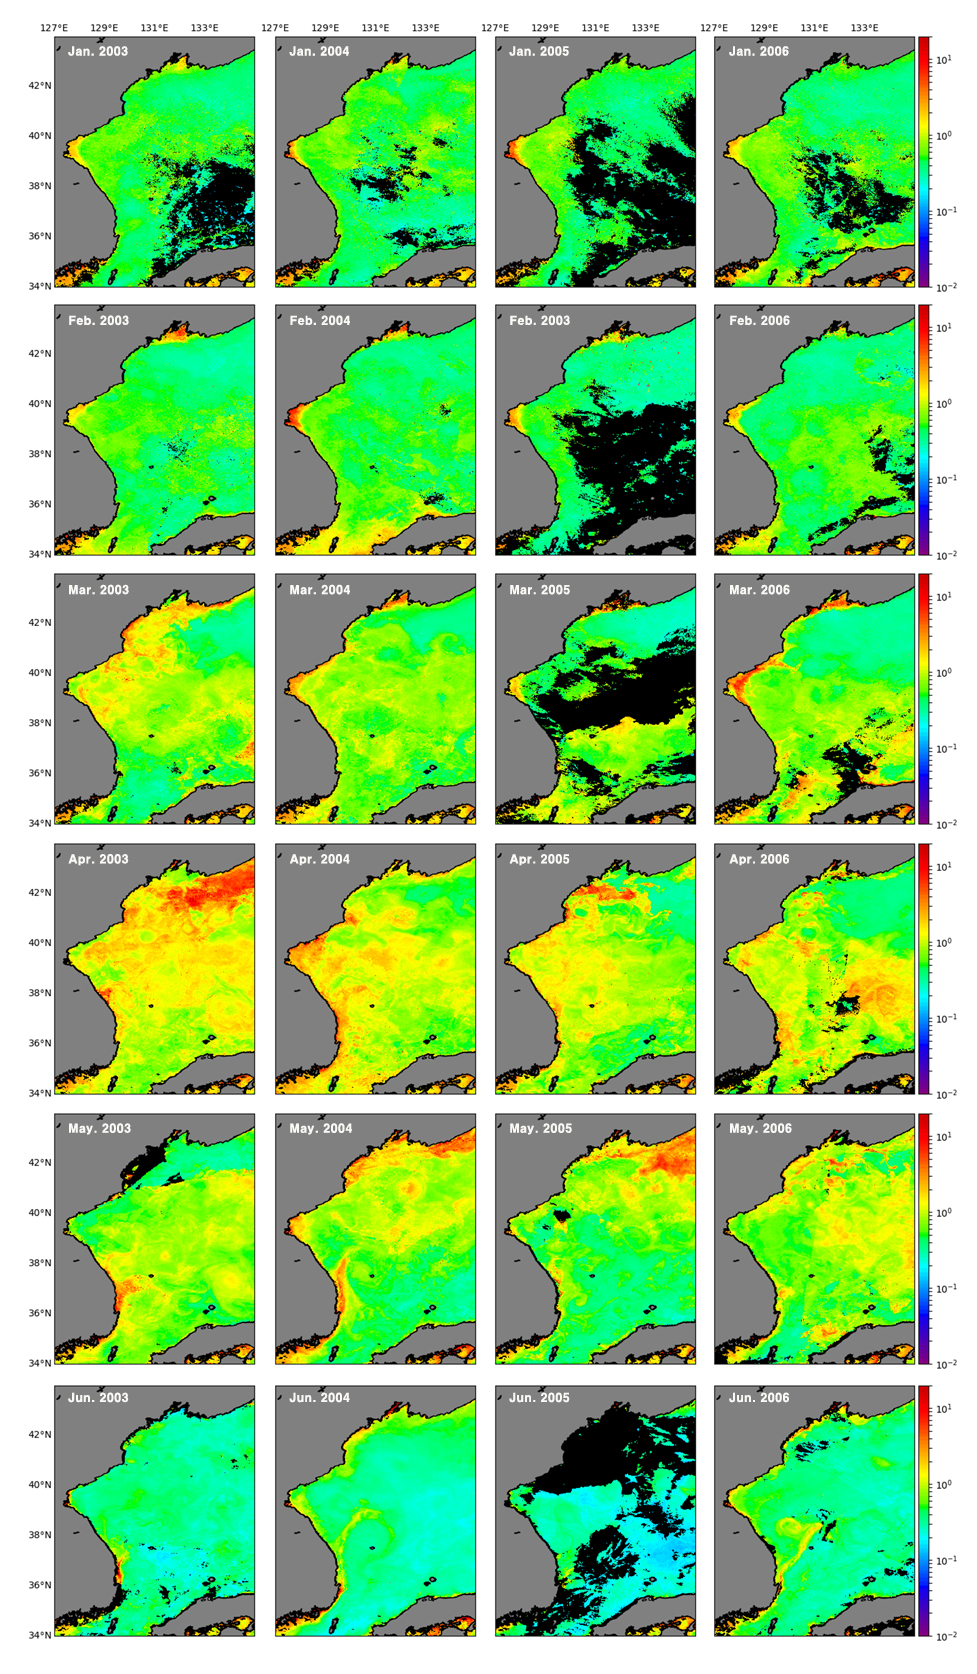
\includegraphics[width=0.8\linewidth]{../images/noname01}
	\caption{The monthly-mean chlorophyll-a distribution in the Korean East Sea, LAC. From 2003 to 2006, January to June. The unit of the color bar is $\rm mg/m^3$.}
	\label{fig:noname01}
\end{figure}
 

\begin{figure}
	\centering
	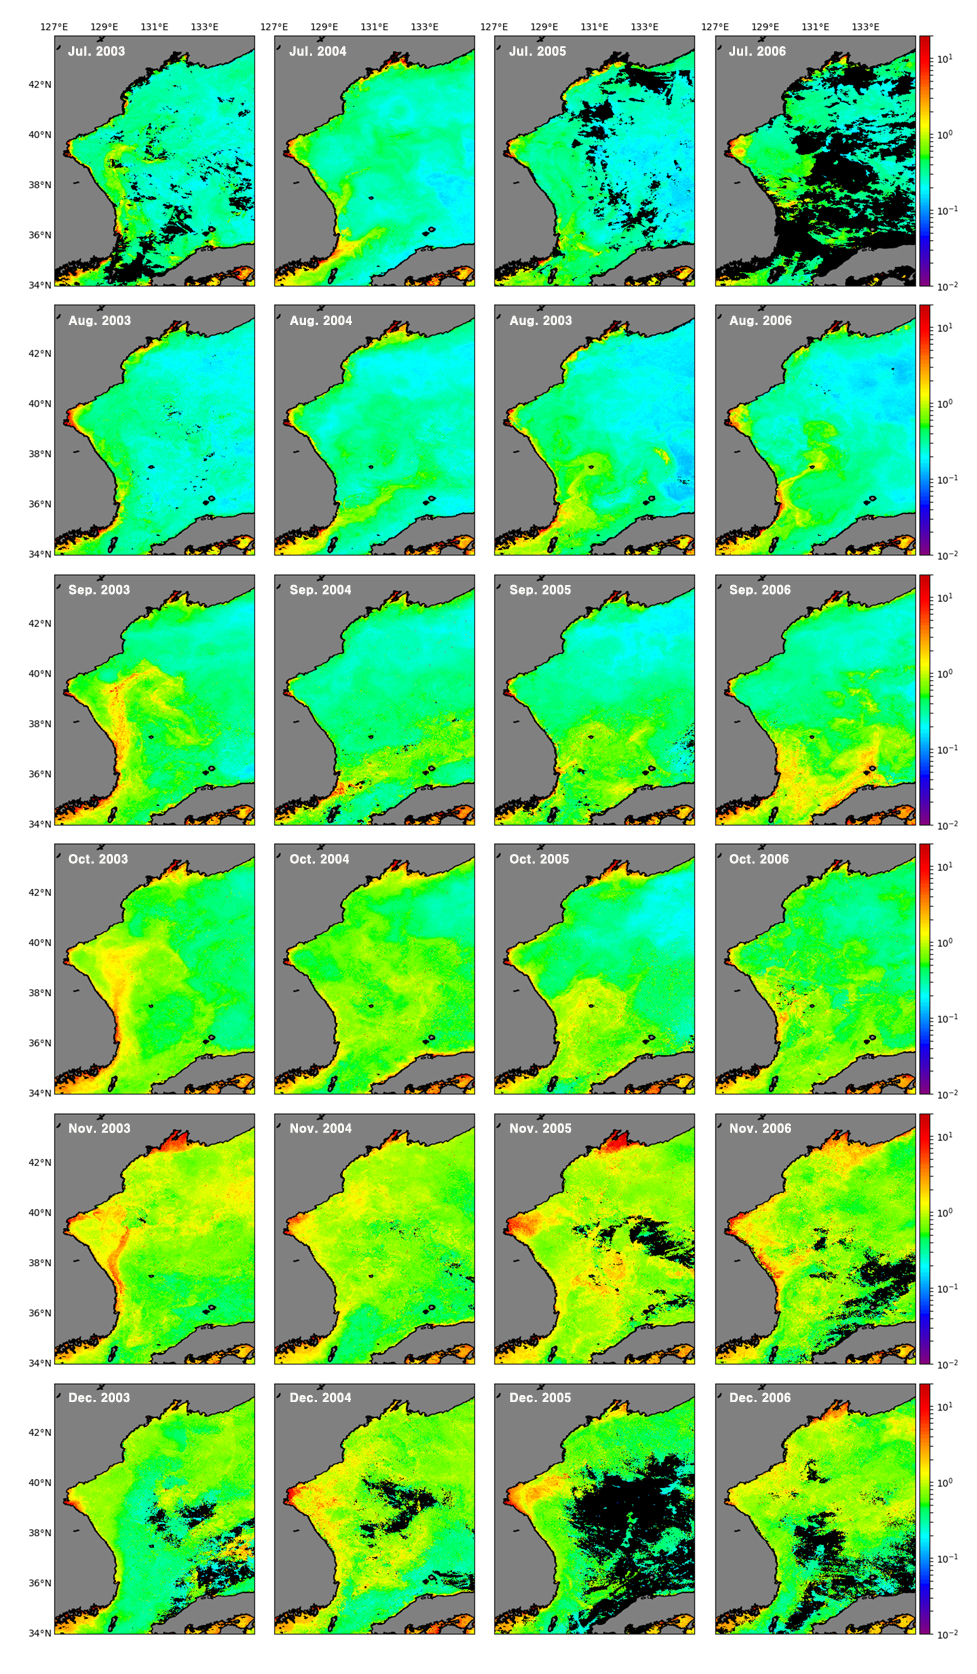
\includegraphics[width=0.8\linewidth]{../images/noname02}
	\caption{The monthly-mean chlorophyll-a distribution in the Korean East Sea, LAC. From 2003 to 2006, July to December. The unit of the color bar is $\rm mg/m^3$.}
	\label{fig:noname02}
\end{figure}

\begin{figure}
	\centering
	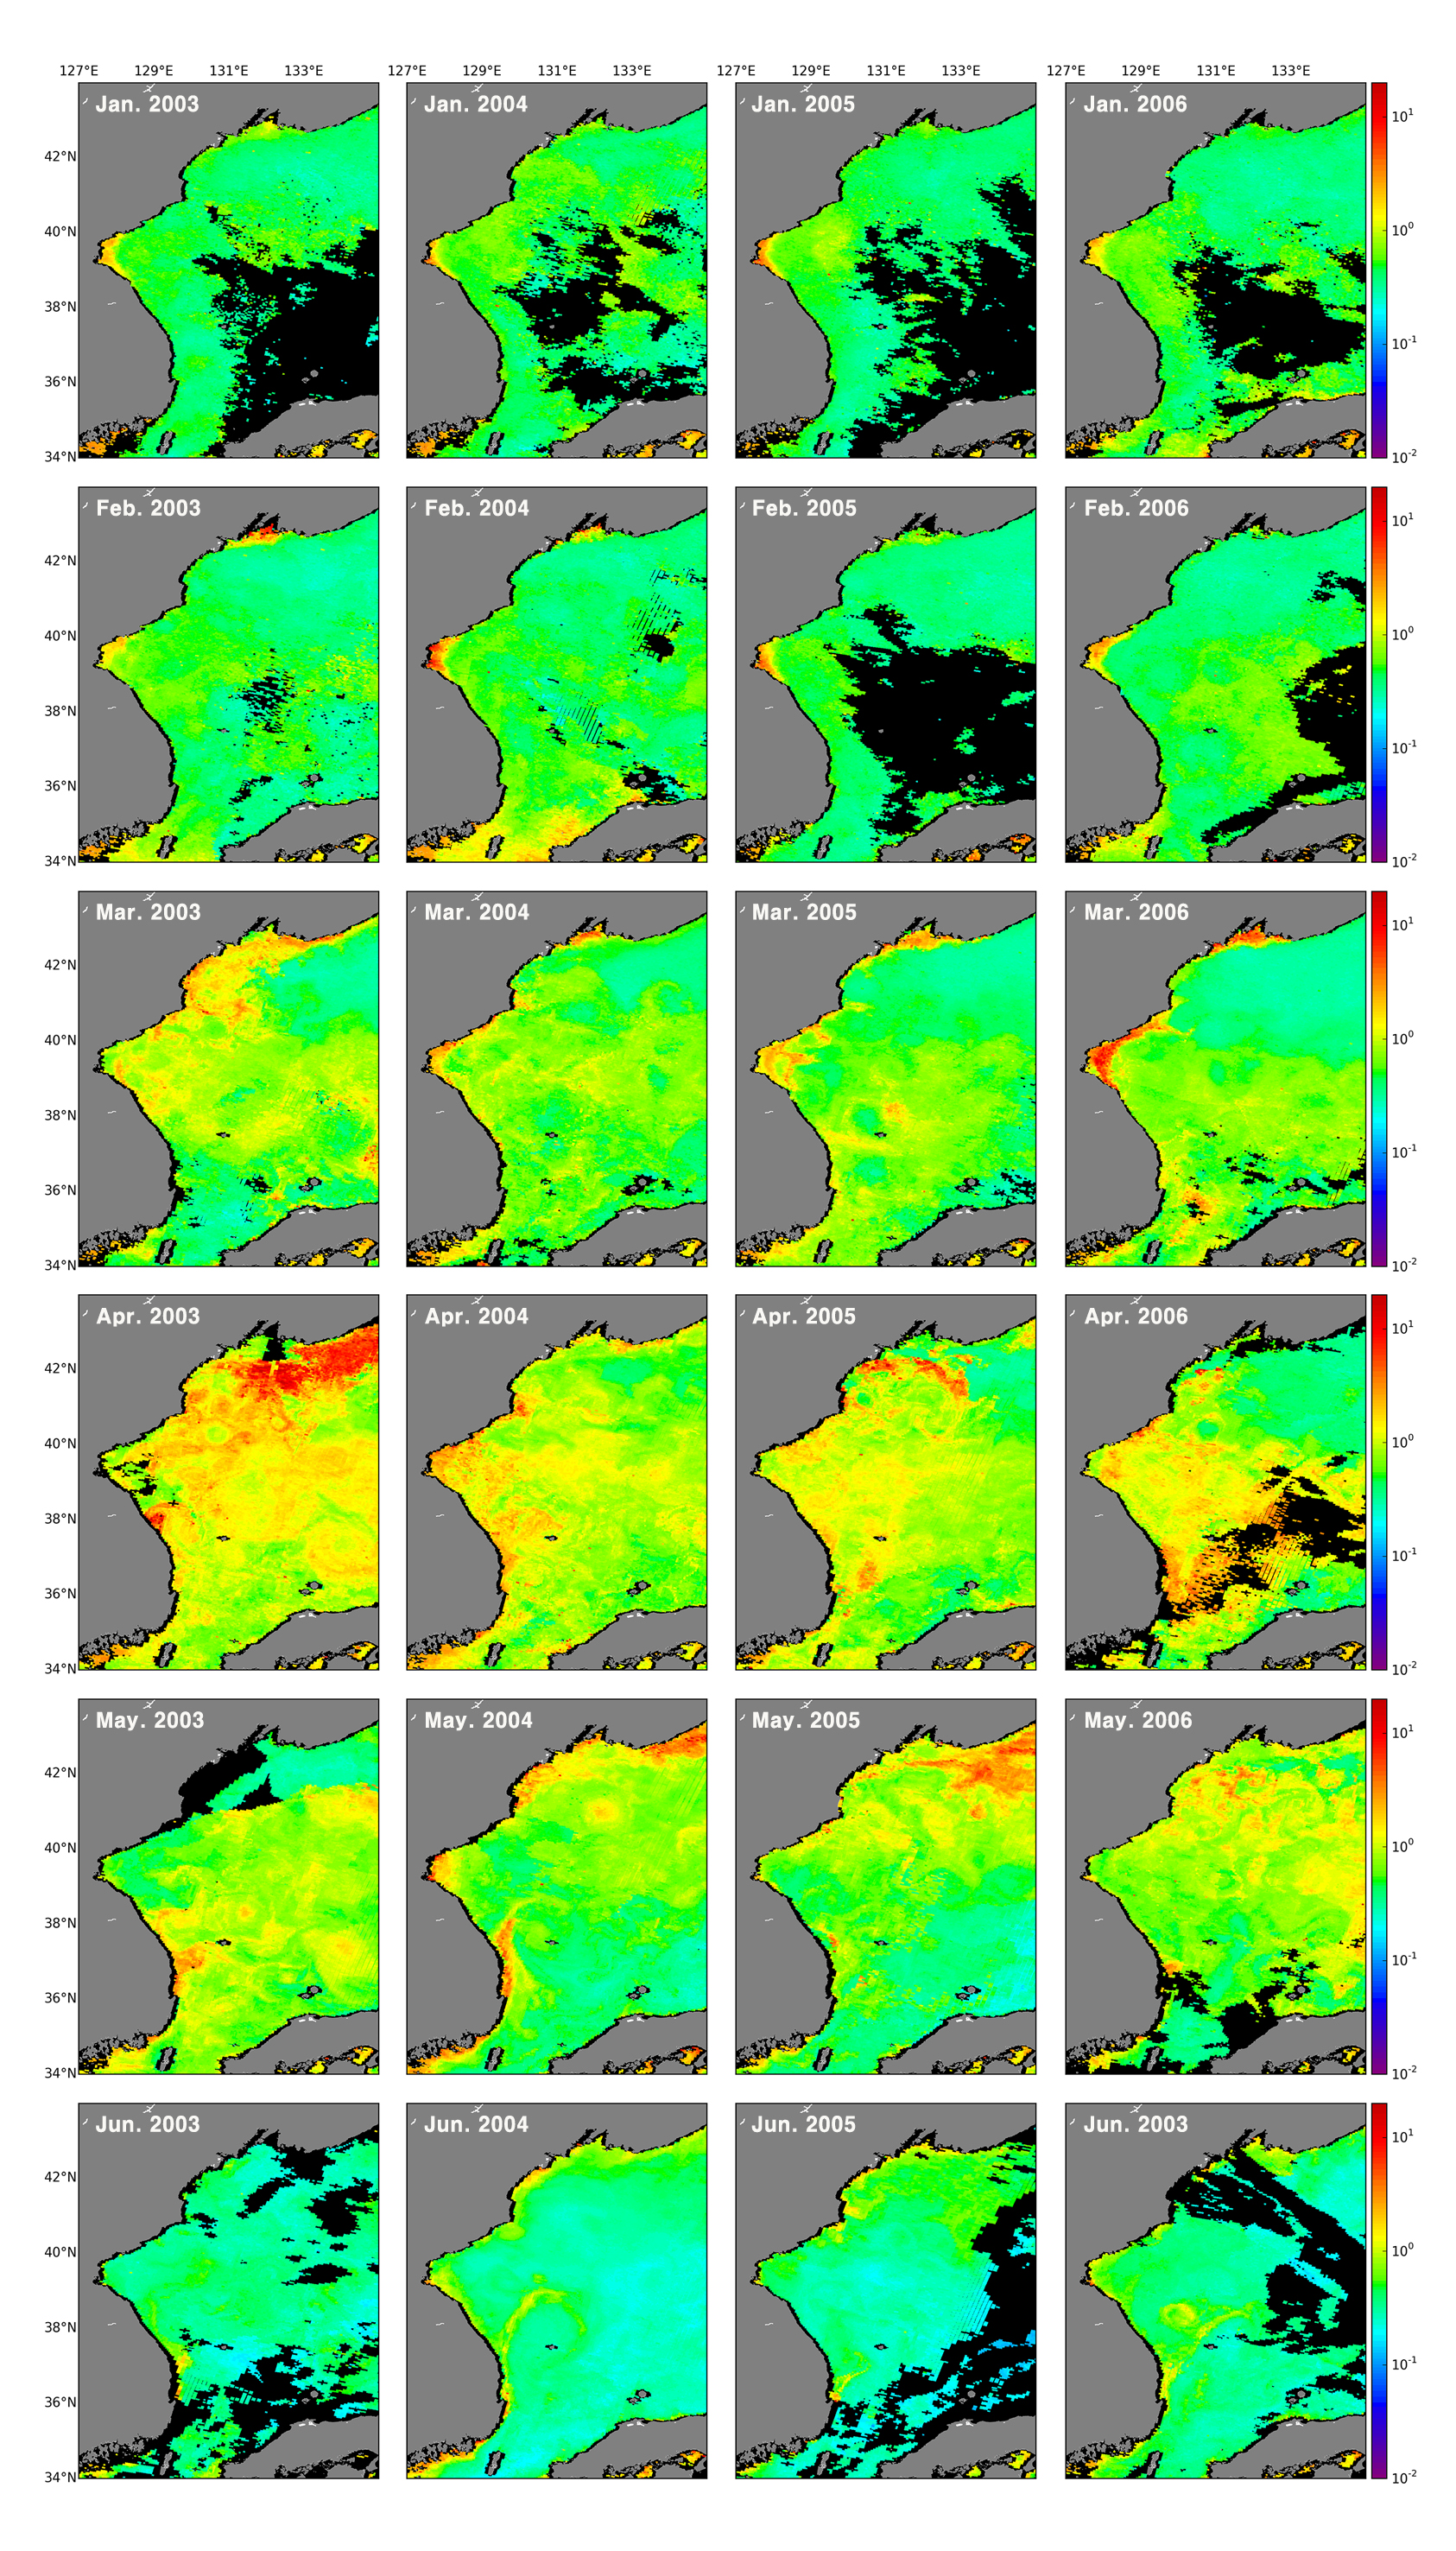
\includegraphics[width=0.8\linewidth]{../images/noname03}
	\caption{The monthly-mean chlorophyll-a distribution in the Korean East Sea, GAC. From 2003 to 2006, January to June. The unit of the color bar is $\rm mg/m^3$.}
	\label{fig:noname03}
\end{figure}

\begin{figure}
	\centering
	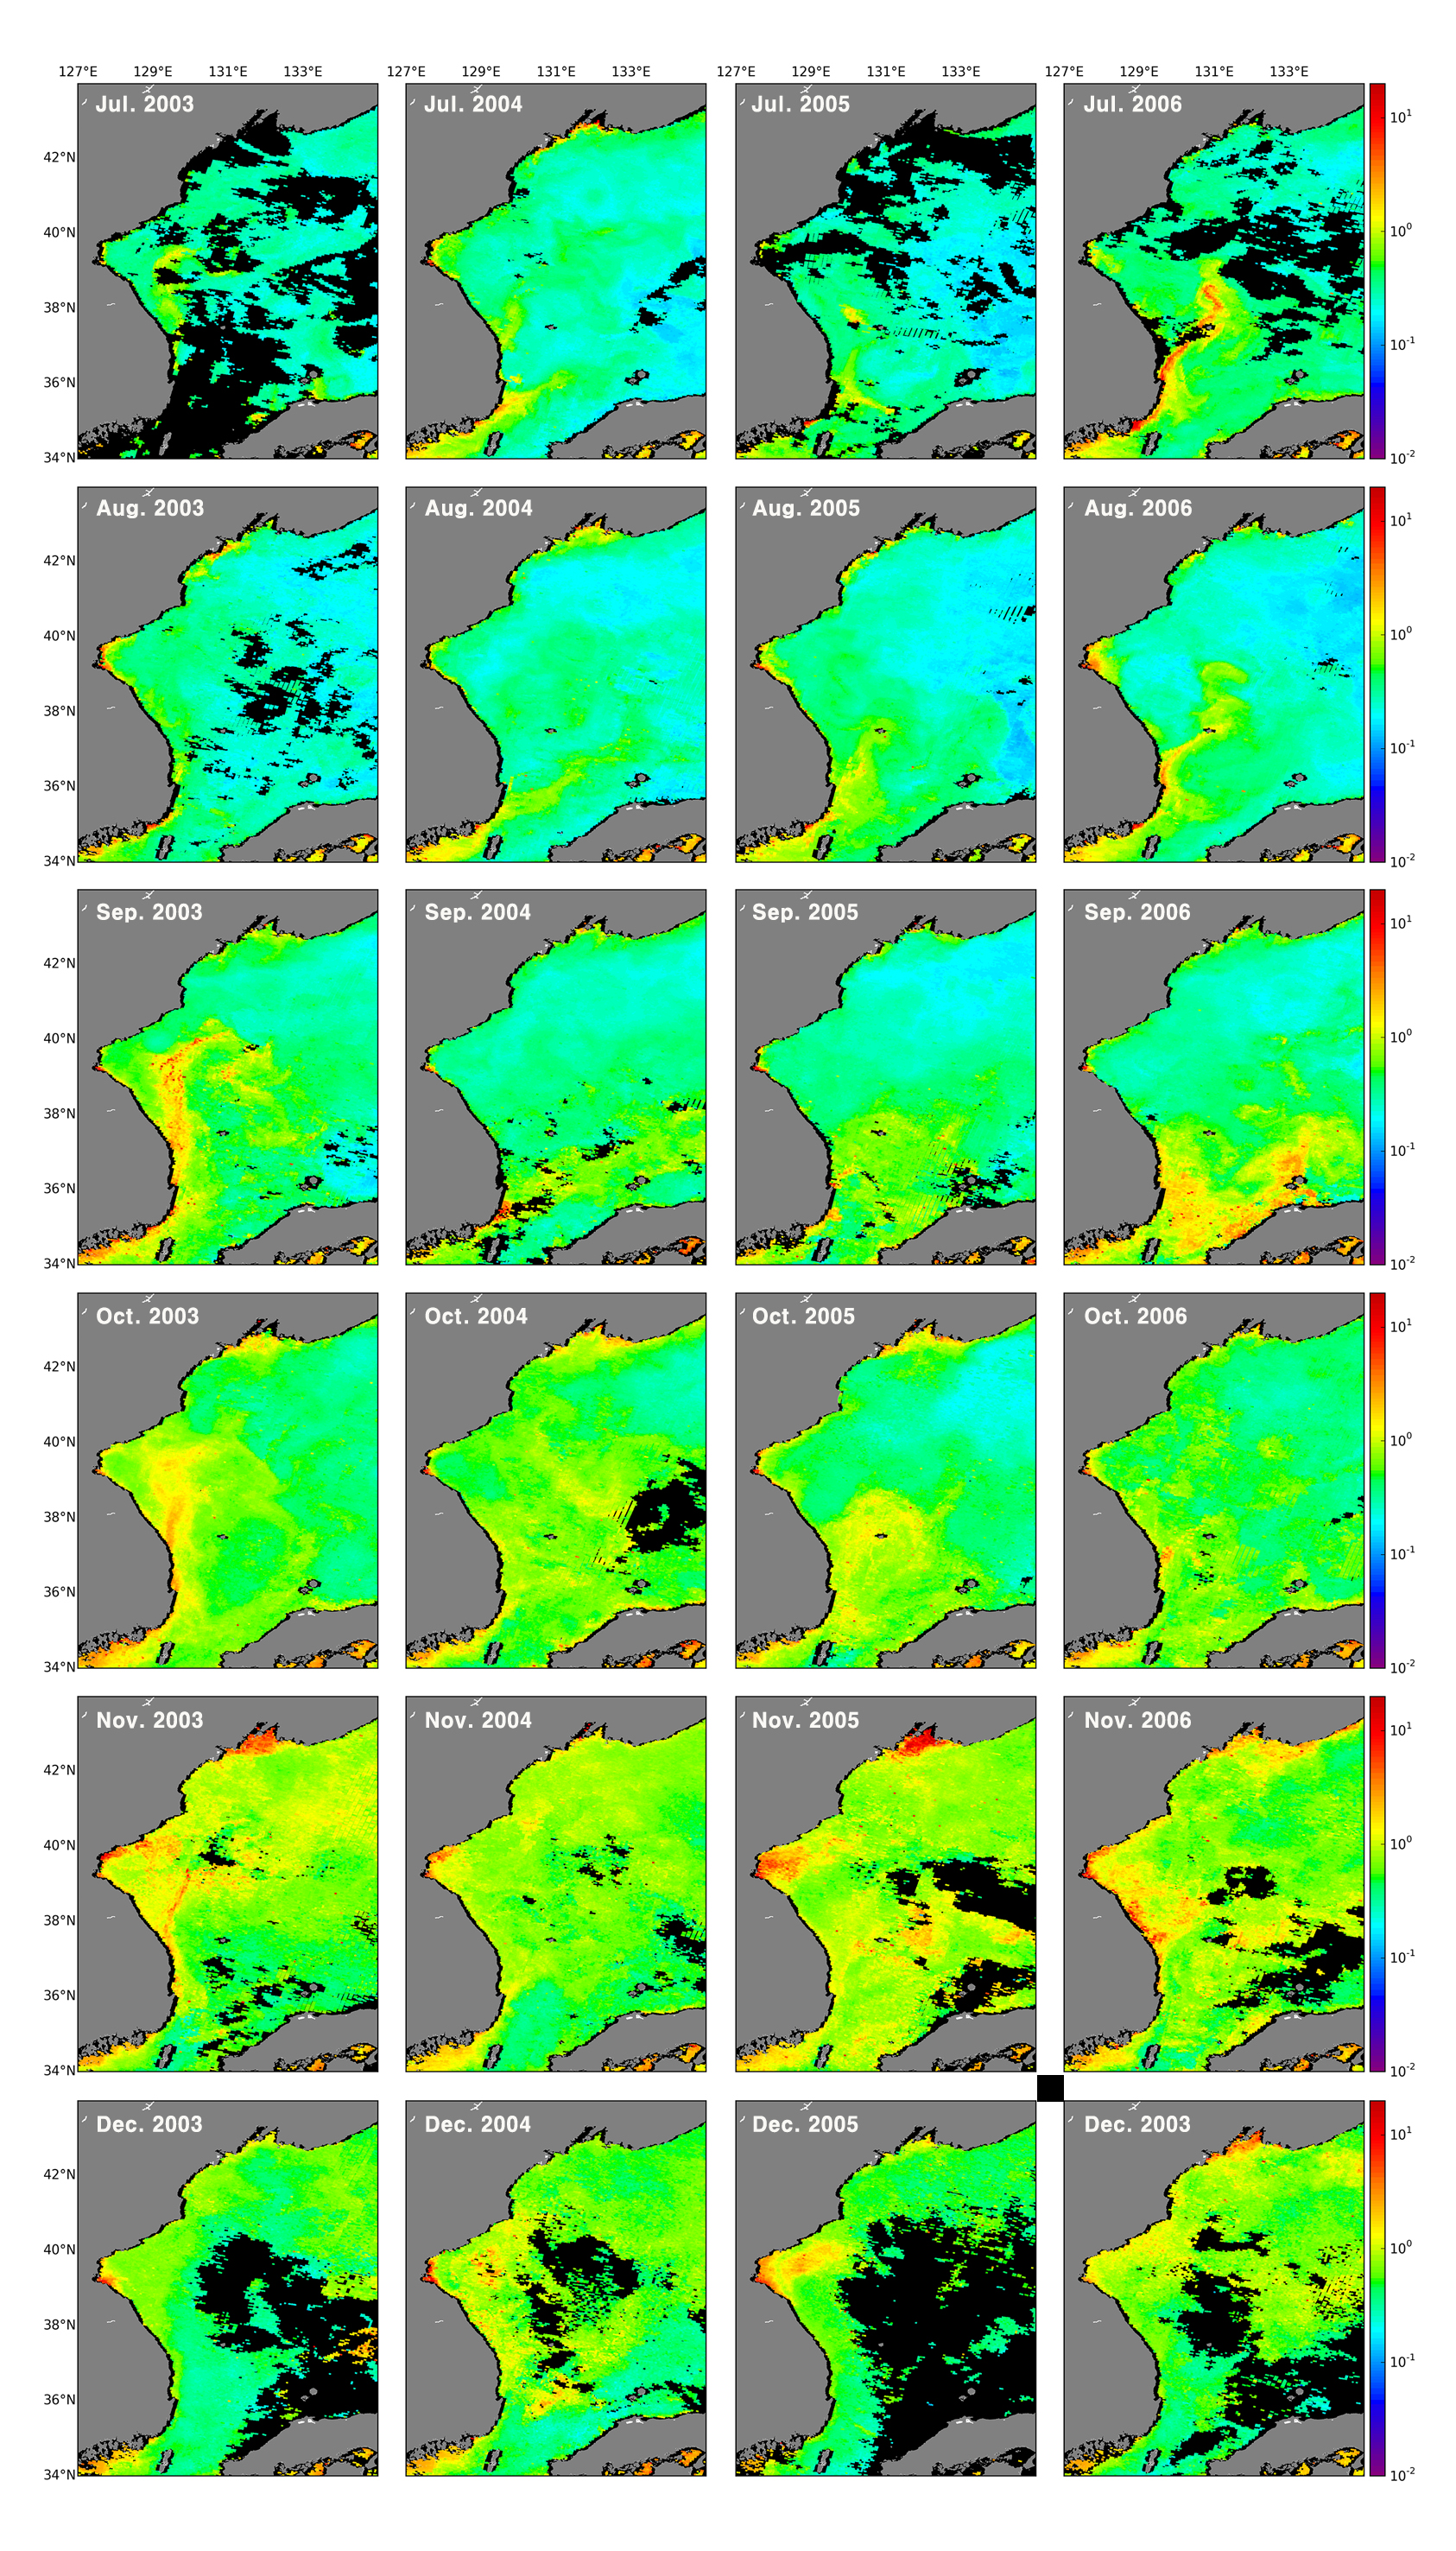
\includegraphics[width=0.8\linewidth]{../images/noname04}
	\caption{The monthly-mean chlorophyll-a distribution in the Korean East Sea, GAC. From 2003 to 2006, July to December. The unit of the color bar is $\rm mg/m^3$.}
	\label{fig:noname04}
\end{figure}
 
\subsection{The Effect of Spatial Resolution on the Data}
 
To find the effect of spatial resolution on the data, we compare the histograms of LAC data and the GAC data of April, 2003. We find that the histogram of GAC data shows more discontinuous shape compared to the LAC data in Figure.9. From the fact that a histogram of real data has continuous shape, it can be inferred that using LAC data is more accurate than using GAC data. The histogram of GAC data also shows more pixels with over 10 mg/m3 of chlorophyll-a concentration with sporadic distribution. These pixels are the speckles from previous researches (Chae, H. J., and Park, K., 2009; Hu, C., Carder, K. L., and Muller-Karger, F. E., 2001) also showing that LAC data is more appropriate for studying chlorophyll-a concentration.
  
  
  Figure 7 The monthly chlorophyll-a mean histogram in the Korean East Sea on April, 2003, (a) LAC (b) GAC.
  
  
   In Figure 10, part of the data with high chlorophyll-a concentration is enlarged to compare between LAC data and GAC data. LAC data has 6 pixels over 10 mg/m3, while GAC data has more than 100 pixels over 10 $\rm mg/m^3$. Such result occurs since one high-concentration value in GAC data affects a large area compared to LAC because of its low resolution.
  In Figure 11, part of the data with speckles is enlarged to compare between LAC data and GAC data. GAC data has a larger size of speckle because it has low resolution. In other words, it has more errors. Even if the speckles of the GAC data has been corrected, it will correct larger area compared to LAC causing a larger gap between the real value. In addition, even with the speckle correction applied using corrected LAC data will be more accurate.
  
  Figure 8. The monthly chlorophyll-a mean distribution in the Korean East Sea on April, 2003, (a) LAC (b) GAC. Enlarged an area with high concentrations of chlorophyll-a
  
  Figure 9. The monthly chlorophyll-a mean distribution in the Korean East Sea on April, 2003, (a) LAC (b) GAC. Enlarged an area with speckles
  
  
  
  

	
\section{Results}
 
\subsection{The Annual Variability of Chlorophyll-a Concentration in the Korean East Sea}
 
The annual variability of chlorophyll-a concentration in the Korean East Sea from 2003 - 2006 is shown in Figure 1, Figure 2. Both the LAC data and the GAC data has similar tendency, showing peaks on spring(April) and fall(November). The maximum/minimum value of LAC and GAC data was each 1.61 $\rm mg/m^3$ / 0.28 $\rm mg/m^3$, and 1.72 $\rm mg/m^3$ / 0.32 $\rm mg/m^3$. The difference between the two data was not ignorable. This infer that the effect of spatial resolution on the data has to be considered.
  
 Figure.
 
The annual variability of 8-day-mean chlorophyll-a concentration in the Korean East Sea from 2003 to 2006 is shown in Figure 3, Figure 4. This result allowed more concrete analysis of the data. The spring peak had 1.2 - 1.3 $\rm mg/m^3$ of chlorophyll-a concentration and was higher than the fall peak which had the value of 0.9 - 1.0 $\rm mg/m^3$. Winter had a higher concentration (0.6 $\rm mg/m^3$) compared to summer (0.4 $\rm mg/m^3$). The chlorophyll-a concentration in the Korean East Sea had clear seasonal differences. Both the LAC data and the GAC data was sufficient to show the seasonal differences. However, even though the 8-day mean data was created using average of 4 years, the time of maximum concentration was different. 

Part of the LAC data (2004 46th 8-day mean, 2005 11th 8-day mean, 2005 31th 8-day mean) had been lost due to satellite failures. The data for these dates were substituted with the average of the adjacent data. This did not have a significant effect on the tendency, so the error was ignorable.
  
  Figure.
 
The monthly-mean chlorophyll-a concentration of LAC from 2003 to 2006 is shown in \ref{fig:noname01} and \ref{fig:noname02}. The monthly-mean chlorophyll-a concentration of GAC from 2003 to 2006 is shown in \ref{fig:noname03} and \ref{fig:noname04}. The grey area is land showing Korea at the west and Japan at the southeast. Red means high concentration than the blue as it can be told from the color bar. Spring (March, April, May) and fall (October, November) show high concentration. The black area is part with no data due to cloud coverage or satellite failures. 
    
\begin{figure}[t]
	\centering
	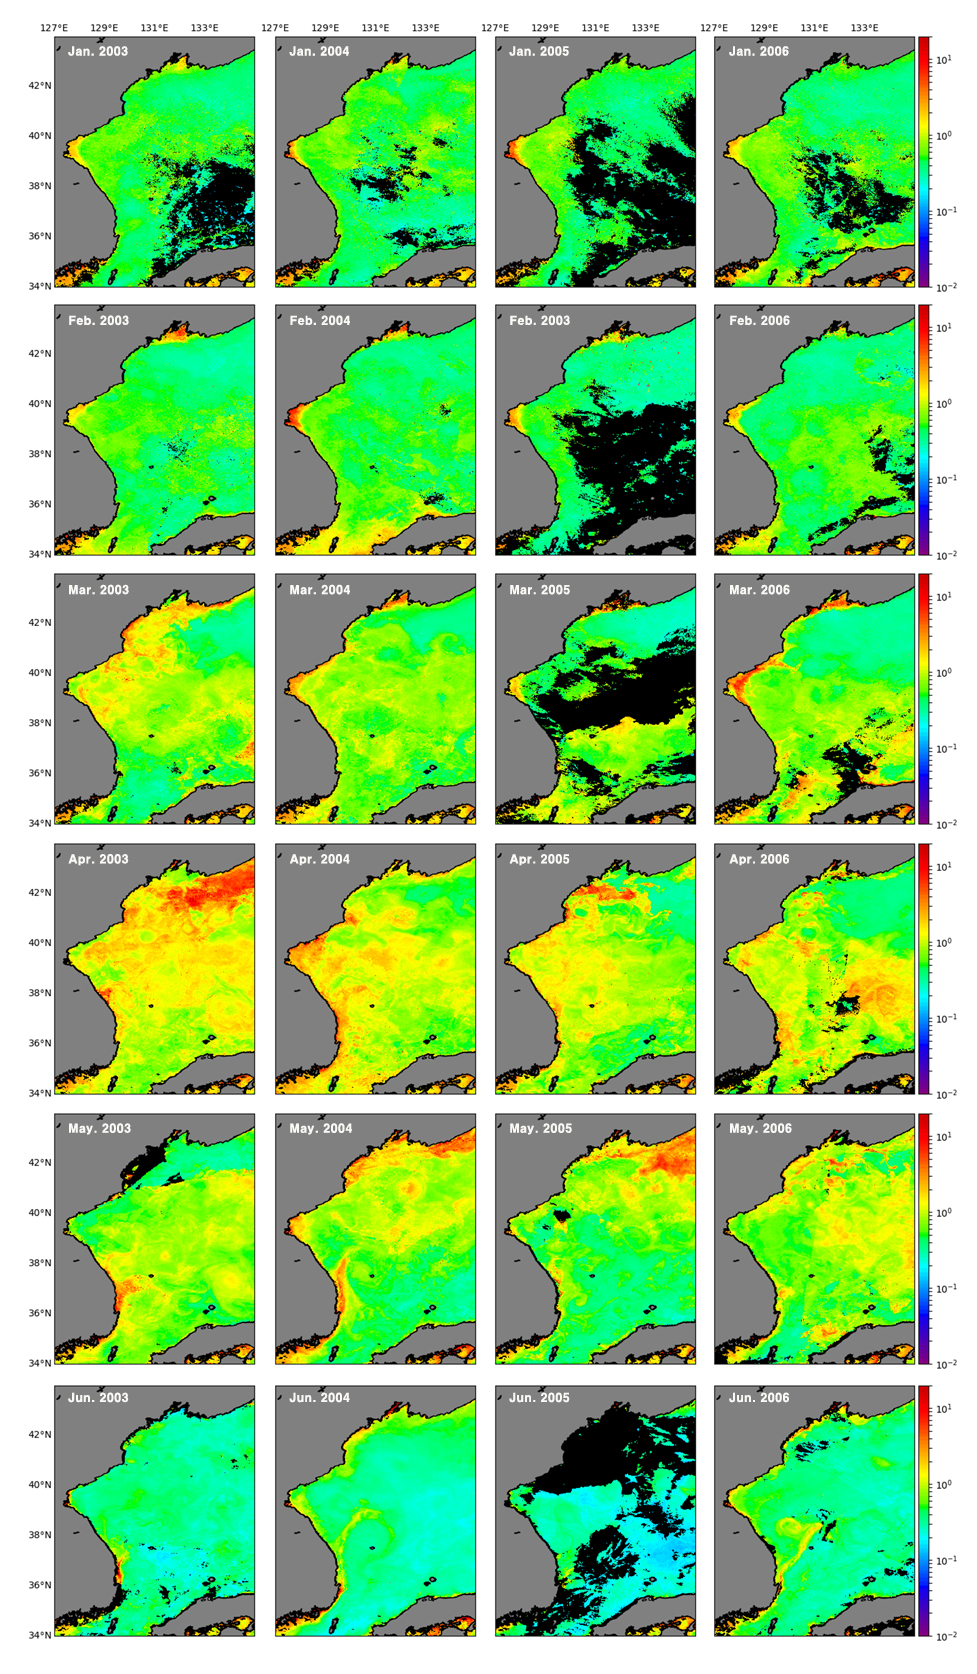
\includegraphics[width=0.8\linewidth]{../images/noname01}\\
	\caption{The monthly-mean chlorophyll-a distribution in the Korean East Sea, LAC. From 2003 to 2006, January to June. The unit of the color bar is $\rm mg/m^3$.}
	\label{fig:noname01}
\end{figure}
 

\begin{figure}
	\centering
	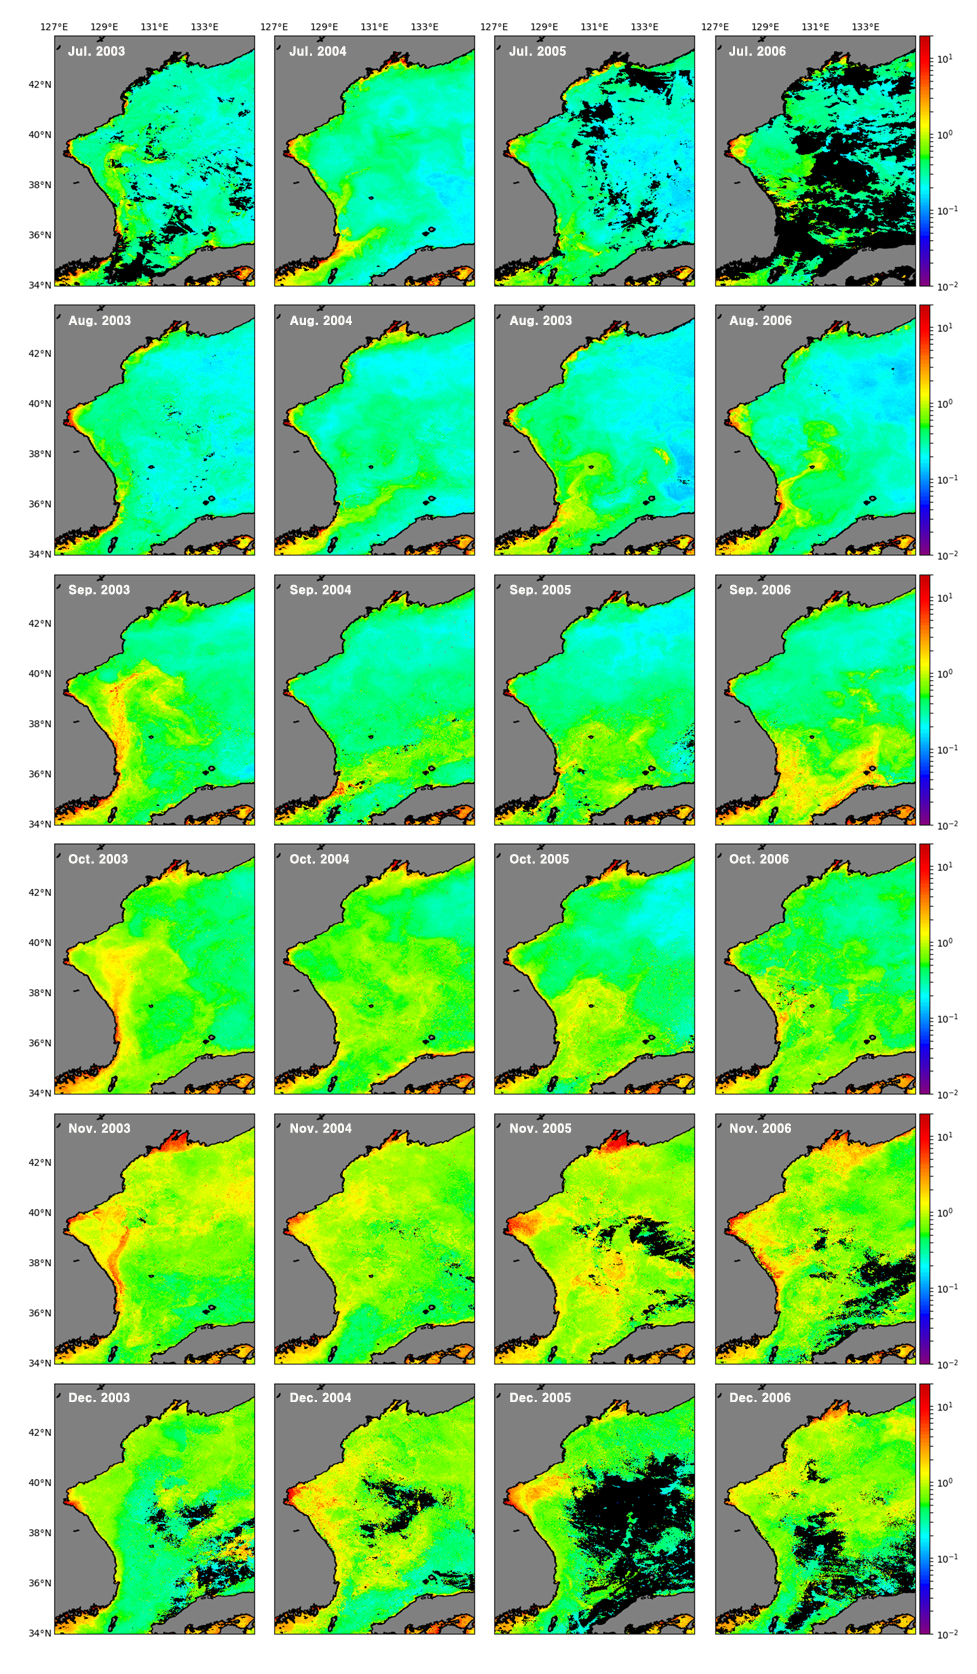
\includegraphics[width=0.8\linewidth]{../images/noname02}
	\caption{The monthly-mean chlorophyll-a distribution in the Korean East Sea, LAC. From 2003 to 2006, July to December. The unit of the color bar is $\rm mg/m^3$.}
	\label{fig:noname02}
\end{figure}

\begin{figure}
	\centering
	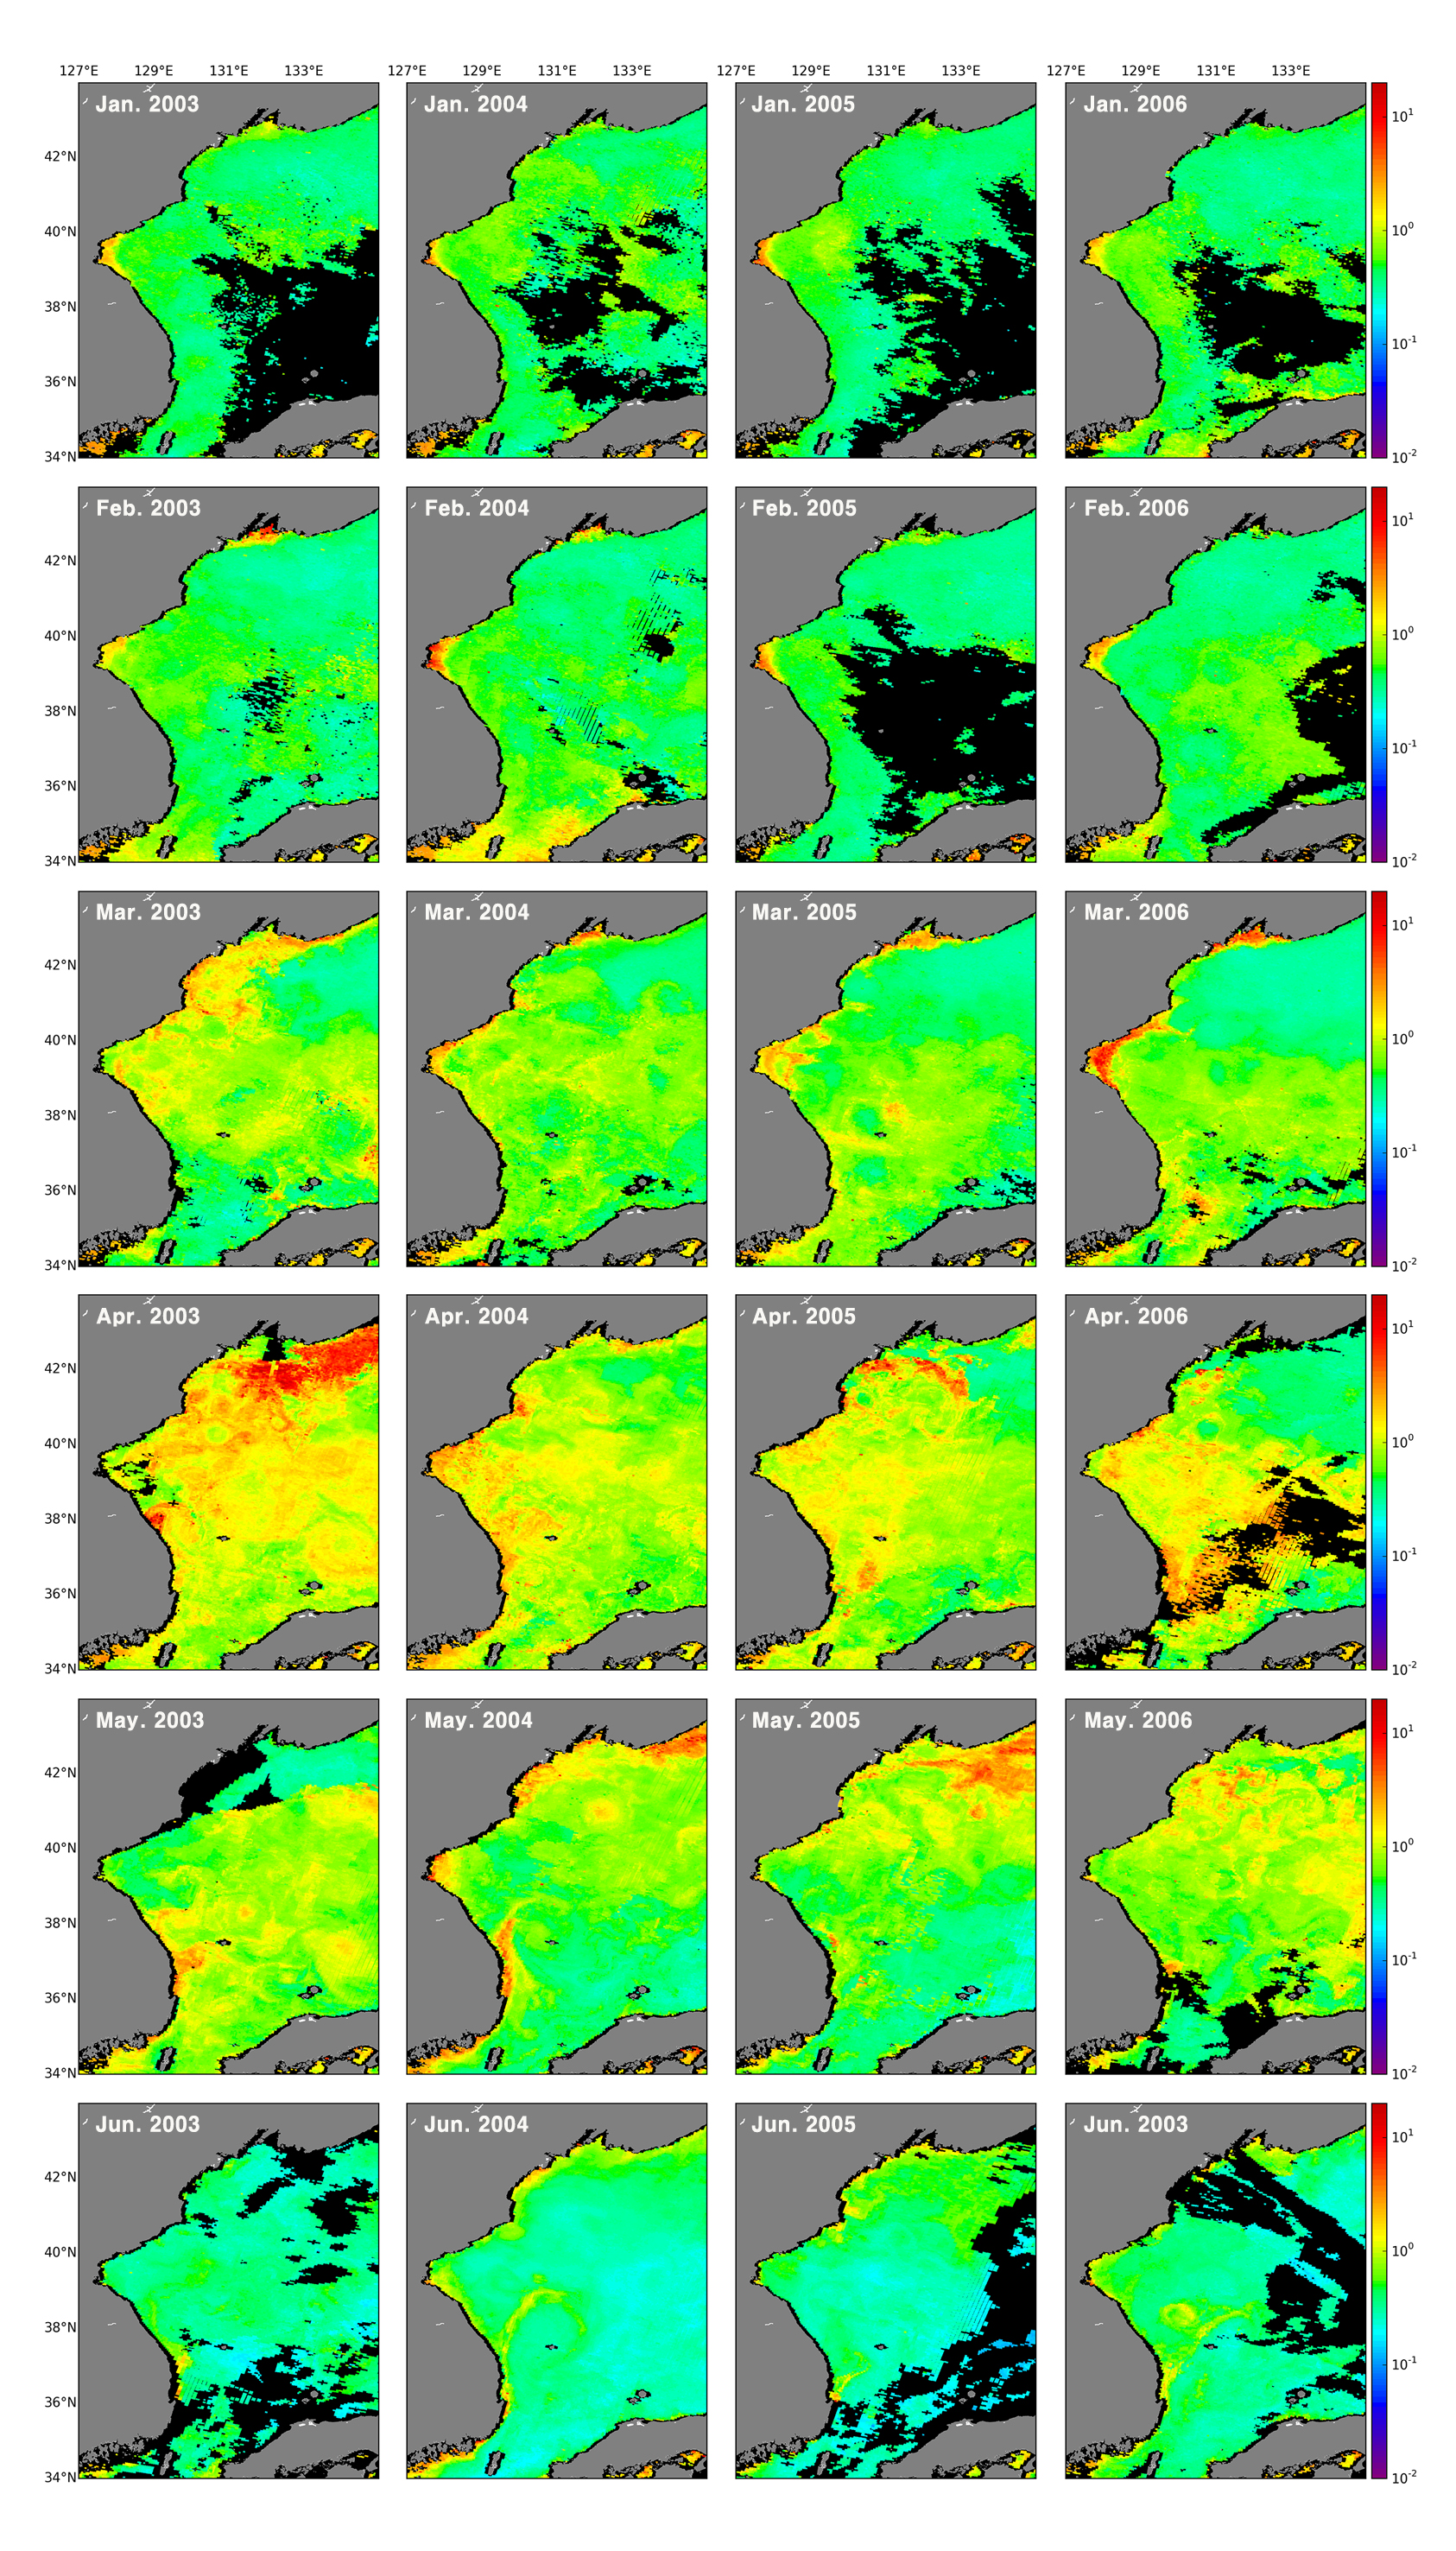
\includegraphics[width=0.8\linewidth]{../images/noname03}
	\caption{The monthly-mean chlorophyll-a distribution in the Korean East Sea, GAC. From 2003 to 2006, January to June. The unit of the color bar is $\rm mg/m^3$.}
	\label{fig:noname03}
\end{figure}

\begin{figure}
	\centering
	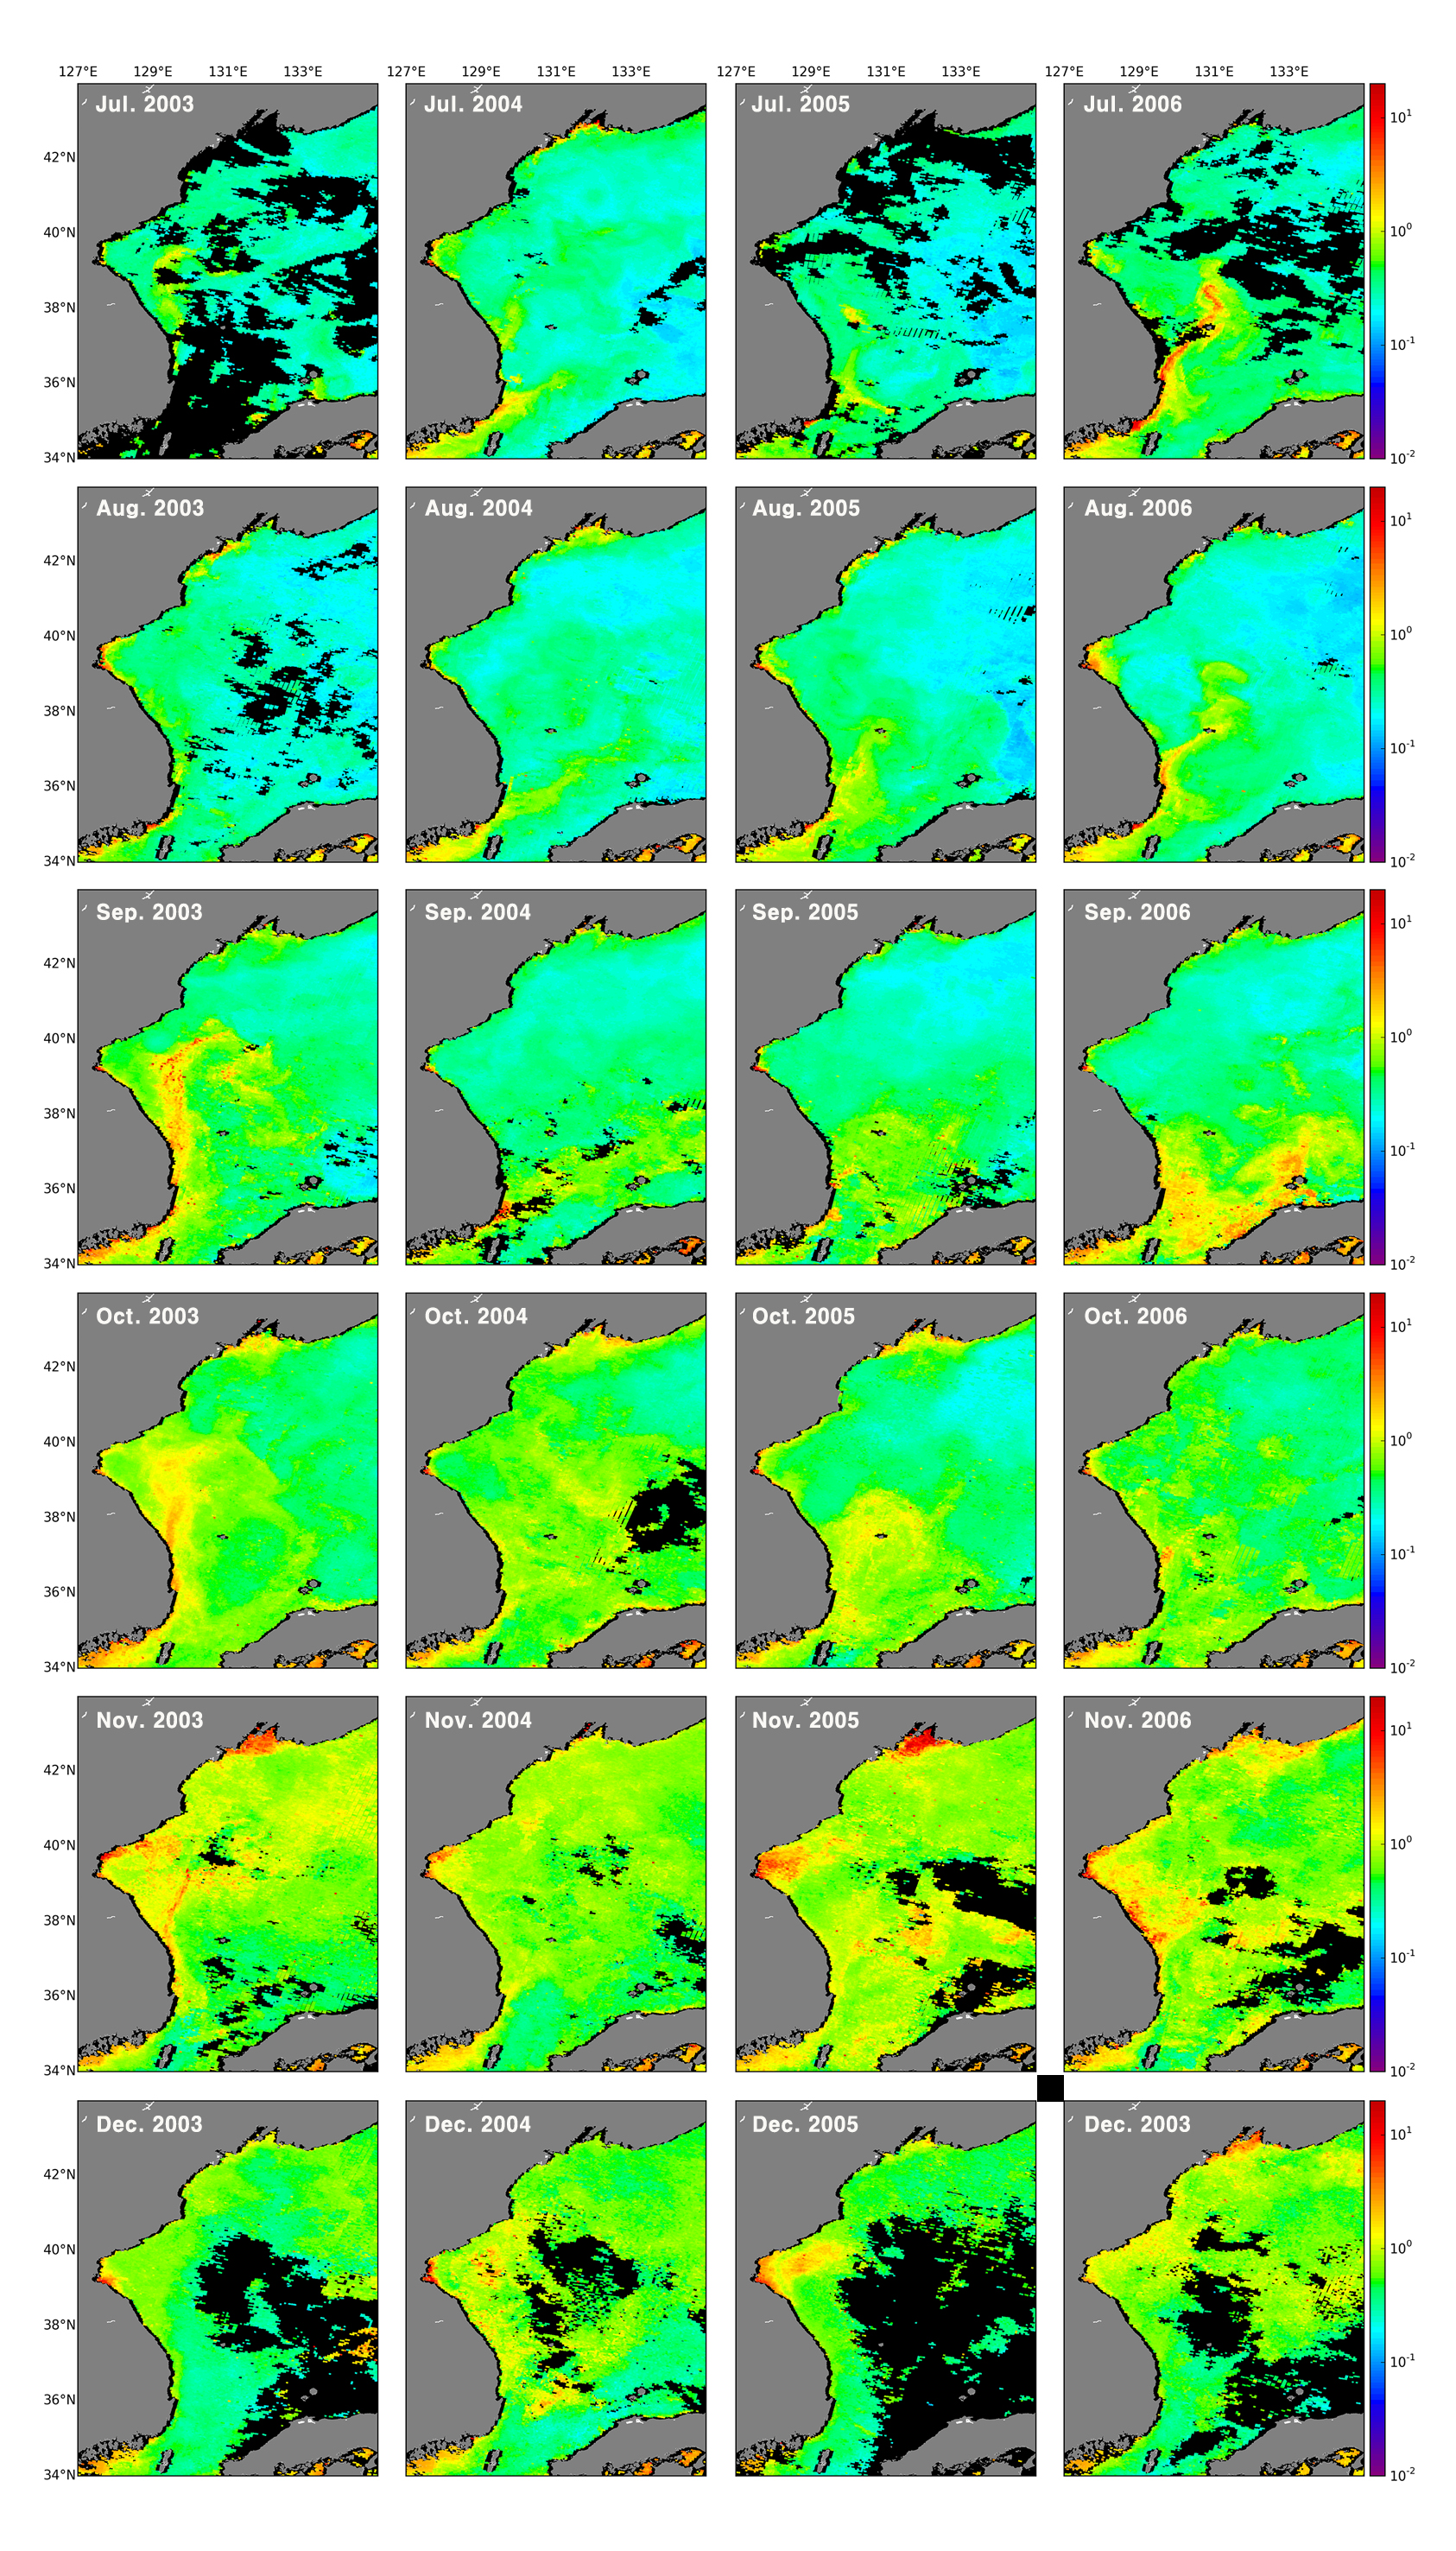
\includegraphics[width=0.8\linewidth]{../images/noname04}
	\caption{The monthly-mean chlorophyll-a distribution in the Korean East Sea, GAC. From 2003 to 2006, July to December. The unit of the color bar is $\rm mg/m^3$.}
	\label{fig:noname04}
\end{figure}
 
\subsection{The Effect of Spatial Resolution on the Data}
 
To find the effect of spatial resolution on the data, we compare the histograms of LAC data and the GAC data of April, 2003. We find that the histogram of GAC data shows more discontinuous shape compared to the LAC data in Figure.9. From the fact that a histogram of real data has continuous shape, it can be inferred that using LAC data is more accurate than using GAC data. The histogram of GAC data also shows more pixels with over 10 mg/m3 of chlorophyll-a concentration with sporadic distribution. These pixels are the speckles from previous researches (Chae, H. J., and Park, K., 2009; Hu, C., Carder, K. L., and Muller-Karger, F. E., 2001) also showing that LAC data is more appropriate for studying chlorophyll-a concentration.
  
  
  Figure 7 The monthly chlorophyll-a mean histogram in the Korean East Sea on April, 2003, (a) LAC (b) GAC.
  
  
   In Figure 10, part of the data with high chlorophyll-a concentration is enlarged to compare between LAC data and GAC data. LAC data has 6 pixels over 10 mg/m3, while GAC data has more than 100 pixels over 10 $\rm mg/m^3$. Such result occurs since one high-concentration value in GAC data affects a large area compared to LAC because of its low resolution.
  In Figure 11, part of the data with speckles is enlarged to compare between LAC data and GAC data. GAC data has a larger size of speckle because it has low resolution. In other words, it has more errors. Even if the speckles of the GAC data has been corrected, it will correct larger area compared to LAC causing a larger gap between the real value. In addition, even with the speckle correction applied using corrected LAC data will be more accurate.
  
  Figure 8. The monthly chlorophyll-a mean distribution in the Korean East Sea on April, 2003, (a) LAC (b) GAC. Enlarged an area with high concentrations of chlorophyll-a
  
  Figure 9. The monthly chlorophyll-a mean distribution in the Korean East Sea on April, 2003, (a) LAC (b) GAC. Enlarged an area with speckles
  
  
  
  

	% Next Section (e.g. Experiment, Linear theory, etc...) 
	% 이외에도 추가로 section마다 파일을 sub 폴더 안에 넣고 여기에서 
	% include 해주면 됩니다.
	% 예시 : methodology.tex을 sub 폴더안에 저장, 이 자리에 
	% \section{Methodology}

\subsection{Acquiring SeaWiFS data}

 This research used SeaWiFS ocean color data to derive chlorophyll-a concentration since SeaWiFS is a satellite that was created to collect global ocean biological data. Moreover, SeaWiFS creates data with two different resolutions that can be compared. However, research on recent years is not possible since SeaWiFS had been activating from September 1997 to December 2010. Table \ref{table01} shows the mission charactoristics of SeaWiFS and Table \ref{table02} shows the Cahracteristics of the DeaWiFS ocean color sensor \cite{hooker1992An}.

 \begin{table}[h]\textwidth
 	\caption{The mission characteristics of SeaWiFS.}
 	\label{table01}
 	\centering
 	\begin{tabular}{c|c}
 		\hline \setlength{\arrayrulewidth}{0.8pt}. 
 	Orbit Type	& Sun Synchronous at 705 km \\ \hline
 	Equator Crossing &	Noon +20 min, descending \\ \hline
 	Orbital Period &	99 minutes  \\ \hline
 	Swath Width &	2,801 km LAC/HRPT (58.3 degrees)  \\ \hline
 	Swath Width &	1,502 km GAC (45 degrees)  \\ \hline
 	Spatial Resolution &	1.1 km LAC, 4.5 km GAC  \\ \hline
 	Real-Time Data Rate &	665 kbps  \\ \hline
 	Revisit Time &	1 day  \\ \hline
 	Digitization &	10 bits  \\ \hline
 	\end{tabular}
 \end{table}

 \begin{table}[h]\textwidth
	\caption{Cahracteristics of the DeaWiFS ocean color sensor.}
	\label{table02}
	\centering
	\begin{tabular}{c|c|c|c|c}
		\hline \setlength{\arrayrulewidth}{0.8pt}. 
		Band	& Wavelength FWHM[nm] & Saturation Radiance & Input Radiance & SNR\\ \hline
		1 & 402-422 & 13.63 & 9.10 & 499 \\ \hline
		2 & 433-453 & 13.25 & 8.41 & 674  \\ \hline
		3 & 480-500 & 10.50 & 6.56 & 667 \\ \hline
		4 & 500-520 & 9.08 & 5.64 & 640  \\ \hline
		5 & 545-565 & 7.44 & 4.57 & 596 \\ \hline
		6 & 660-680 & 4.20 & 2.46 & 442  \\ \hline
		7 & 745-785 & 3.00 & 1.61 & 455 \\ \hline
		8 & 845-885 & 2.13 & 1.09 & 467  \\ \hline

	\end{tabular}
\end{table}
 
 The SeaWiFS Level 2 data of chlorophyll-a was downloaded from NASA Ocean Color Web. Processing Level 1 data to Level 2 data was done by NASA, using NASA SeaDAS program. NASA SeaDAS uses two algorithms to create chlorophyll-a concentration data from the Level 1 data of remote sensing reflectance($\rm R_{rs}$); these algorithms are the OCx band ratio algorithm and the color index(CI) algorithm of Hu. 
 The OCx band ratio algorithm use the ratio of two bands in a fourth-order polynomial equation in a relation with chlorophyll-a It can be expressed as the following equation \ref{eq001}.
 
 \begin{equation}
 {\rm log_{10} (chlor_a) = a_0 + \sum_{i=1}^4 a_i ~ log_{10} \left( \frac{(R_{rs}(\lambda_{blue})}{(R_{rs}(\lambda_{green})} \right) ^i }
 \label{eq001}
 \end{equation}
 
The coefficients $\rm a_0$ - $\rm a_4$ are values for each sensor acquired from experiments. The OCx algorithm was proved to be accurate by O’Reilly et. al\cite{o2000ocean}. The CI algorithm uses three bands and can be expressed as the following equation.
The $\rm {\lambda}_{blue}$, $\rm {\lambda}_{green}$, $\rm {\lambda}_{red}$ are wavelengths closest to 443 $\rm nm$, 555 $\rm nm$ and 670 $\rm nm$, different for each sensor. According to Hu, C., Lee, Z., and Franz, B., for the lower concentration of chlorophyll-a (less than 0.25 $\rm mg/m^3$), it is more accurate to use CI algorithm \cite{hu2012chlorophyll}. The NASA SeaDAS software uses CI algorithm for chlorophyll retrievals below 0.15 $\rm mg/m^3$, and OCx band ratio algorithm for retrievals above 0.2 $\rm mg/m^3$. For the concentration between 0.15 $\rm mg/m^3$ and 0.2 $\rm mg/m^3$, it blends both algorithm.
The area of interest was chosen as 32.31°N - 45.00°N, 126.74°E - 135.00°E which covers the whole East Sea near Korea. The Yellow Sea is not covered in this research because it is too shallow for the algorithms to be applied. The dates of the data were chosen from the year 2003 to 2006. This is because from 2007, the number of data files decreases significantly due to the errors generated in the satellite. 


 \subsection{Deriving Chlorophyll-a Concentration using LAC data and GAC data}
 
  NASA SeaDAS is used to process the level 2 data of chlorophyll-a to level 3 data of monthly-mean/ 8-day-mean of chlorophyll-a concentration data. Monthly-mean data is created to show the overall tendency, while 8-day-mean data is created to see more specific tendency. Simple average method had been used to create the mean files. This method sum pixel values of chlorophyll-a at the same location and divide it by the number of data that has been compiled. This process also gives latitude longitude value to the pixels, creating a Standard Mapped Image(SMI). Chae, H. J., & Park, K. (2009) used weighted average method to process data. However, according to Park, K. A., Park, J. E., Lee, M. S., & Kang, C. K. (2012), both the weighted average method and the simple average method are suitable for processing SeaWiFS data in East Sea. In addition, we use the more general method which is the simple average method.
 Since running each process using SeaDAS is inconvenient, so we automate the process by using python batch processing. This commands SeaDAS to repeat the process. Python can also create png files from the SMI. We use the obtained monthly-mean and 8-day-mean data to find the annual variability of chlorophyll-a concentration.
 The effect of spatial resolution on the data was also progressed. The histograms for chlorophyll-a concentration were compared between LAC data and GAC data. Then, the SMI data itself was enlarged to find the difference between them.
  와 같이 작성
	%%%% 주의
	%%%% 파일이 나뉠 때마다 자동으로 페이지넘김(\clearpage)가 됩니다. 
	%%%% 따라서 subsection을 나누는 용도로는 사용하지 마십시오.
	%%%% \include{sub/experiment} 와 같이...


	\section{Discussion}
Spring(April) and fall(November) each had 1.2 ~ 1.3 mg/m3, 0.9 ~ 1.0 mg/m3 of chlorophyll-a concentrations which was higher than the other seasons showing similarities with the result of Yamada, K., Ishizaka, J., Yoo, S., Kim, H. C., & Chiba, S. (2004). Analysis of annual variability with the temporal resolution increased to 8-day-mean data showed winter (December, January, February) had higher concentration compared to summer (June, July, August), each with the values of 0.6 mg/m3 and 0.4 mg/m3. This conclude that the Korean East Sea shows clear seasonal differences.

In a perspective of spatial resolution, both the LAC data and the GAC data were suitable for research on the chlorophyll-a concentration variability in the Korean East Sea. However, histogram analysis showed that GAC data had more speckles compared to LAC data. The pixel analysis of chlorophyll-a concentration data on April, 2003 also showed that even with the speckle correction it is more accurate to use LAC data because of its high resolution.

The limit of this research is that speckle errors were not corrected causing the concentration values to be higher than the in-situ data. Moreover, the in-situ data of the area of interest was not measured in this research so it could not directly show whether the LAC data or the GAC data is more accurate. Further research will compare the processed data of LAC and GAC with the in-situ data from previous researches.
 % Conclusion
	
	%\include{sub/appendix} % Appendix가 없는 경우 주석처리하십시오
	
	\bibliography{bibfile} % 참고문헌
	% BibTeX 코드 쉽게 얻어오는 방법 %
	% Google Scholar 에서 검색한 결과에서 `인용'을 클릭한다.
	% BibTeX 코드를 얻고자 한다면, 하단의 `BibTeX' 을 클릭.
	% 코드가 나온다. Ctrl+A, Ctrl+C로 복사, bibfile에 붙여넣기.
	
	%\include{sub/summary} % Summary
	%(영어로 작성한 학생은 이 부분을 주석 처리하십시오.)
	
	%-----------------------------------------------------
%   감사의 글
%-----------------------------------------------------
\begin{acknowledgements}
\addcontentsline{toc}{section}{감사의 글}  %%% TOC에 표시
정말 감사합니다.
\end{acknowledgements}

%-----------------------------------------------------
%   연구활동 
%-----------------------------------------------------
\begin{researches}
\addcontentsline{toc}{section}{연구활동}  %%% TOC에 표시
\begin{itemize}
\item{2011학년도 교내 R\&E 발표대회에서 장려상 수상}
\item{2012학년도 교내 R\&E 발표대회에서 장려상 수상}
\item{2013학년도 교내 R\&E 발표대회에서 장려상 수상}
\item{2014학년도 교내 R\&E 발표대회에서 장려상 수상}
\item{2015학년도 교내 R\&E 발표대회에서 장려상 수상}
\item{2016학년도 교내 R\&E 발표대회에서 장려상 수상}
\item{2017학년도 교내 R\&E 발표대회에서 장려상 수상}
\item{2018학년도 교내 R\&E 발표대회에서 장려상 수상}
\item{2019년 노벨 물리학상 수상}
\end{itemize}
\end{researches} % 감사의 글 & 연구활동
\end{document}